%% LaTeX2e class for student theses
%% sections/preliminary.tex
%% 
%% Karlsruhe Institute of Technology
%% Institute for Program Structures and Data Organization
%% Chair for Software Design and Quality (SDQ)
%%
%% Dr.-Ing. Erik Burger
%% burger@kit.edu
%%
%% Version 1.1, 2014-11-21

\chapter{Related Work}
\label{ch:Related Work}
This chapter introduces related and previous works in the realm of language identification and how their approaches differ from the ones employed in the following chapters.

\chapter{Fundamentals}
\label{ch:fund}

The following chapter will define and explain terms and concepts used throughout this thesis, as to make understanding of the following chapters easier.

\section{Janus Recognition Toolkit (jrtk)}
\label{sec:fund:jrtk}
The Janus Recognition Toolkit (jrtk) also known as just ``Janus'' is a general-purpose speech recognition toolkit developed in joint cooperation by both the Carnegie Mellon University Interactive Systems Lab and the Karlsruhe Institute of Technology Interactive Systems Lab~\cite{lavie1997janus}. Part of janus and the jrtk are a speech-to-speech translation system which includes Janus-SR the speech recognition component, the main part of janus used in this thesis. 

Developed to be flexible and extensible, the jrtk can be seen as a programmable shell with janus functionality being accessible through objects in the tcl/tk scripting language. It features the IBIS decoder, that uses Hidden Markov Models for acoustic modeling in general, although in this thesis we used a neural network as our speech recognizer to generate the input features required by our Language ID network.

This thesis makes extensive use of the jrtk's and tcl/tk's scripting capabilities to be able to pre-process speech audio files for further use by our experimental setup. It also uses tcl/tk scripts and it's janus API functionality in the development of our smoothing and evaluation scripts as can be seen in Ch.~\ref{ch:eval}.
\section{Neural Networks}
\label{sec:fund:NN}
Artificial Neural Networks today are used in many different fields: from image recognition/face recognition in~\cite{lawrence1997face} to Natural Language Processing in~\cite{collobert2008unified} and, as relevant to this thesis, to Speech Recognition and very successfully as in~\cite{hinton2012deep}. It has also been used in the realm of Language Identification, which will be described in Sec.~\ref{sec:fund:work}. This section will provide fundamental knowledge of how neural networks work and how to train them, to make the understanding of later chapters easier for the reader. The information in this section is based mostly on~\cite{haykin2004comprehensive}, ~\cite{Goodfellow-et-al-2016} and~\cite{deeplearning-online}


\subsection{General Setup}
\label{sec:fund:general}
Neural Networks are based on collections of small ''neural units``  working together in tandem. The neuron's behavior can be loosely linked to the brain's axons. Each neuron is connected with others and a neuron is ''stimulated`` by input on these connections and then decides on its own activation, or stimulation, by using a summation, or threshold, function with a certain limit to decide if the neuron ''fires`` and its own activation is propagated through the network to adjacent units. By changing weigths and activation thresholds in the network its output changes, therefore the possible adjustable parameter set \(\Theta\) for a neural network includes all the weights for all neurons as well as all thresholds for the activation functions in each neuron.

\subsection{Artificial Neuron}
\label{sec:fund:AN}

An artificial neuron, or perceptron in its most basic form, is a mathematical function that consists of four parameters that can be adjusted independently from each other:
\begin{itemize}
\item \(w_i\) the input weights for all inputs
\item \(\Sigma\) the transfer function for summation of the weighted inputs
\item \(\varphi\) the activation function that calculates the output value \(y_k\) basend on the transfer input and the threshold
\item \(\theta\) the threshold which defines when the neuron activates.
\end{itemize}

This means an artificial neuron with output \(y_k\) is the function~\ref{eq:an}. Many of these neurons coupled together (via the output of a neuron on a previous layer becoming the input for one on the current layer), make an Artificial Neural Network as used in this thesis. A schematic drawing of this can be seen in Fig.~\ref{fig:neuron}.

\begin{equation}
y_k = \varphi(\sum_{j=0}^{m} w_{kj}x_j) - \theta_j
\label{eq:an}
\end{equation}

\begin{figure}[h!]
\label{fig:neuron}
\caption{A schematic drawing of a Neuron and it's parameters}
\centering
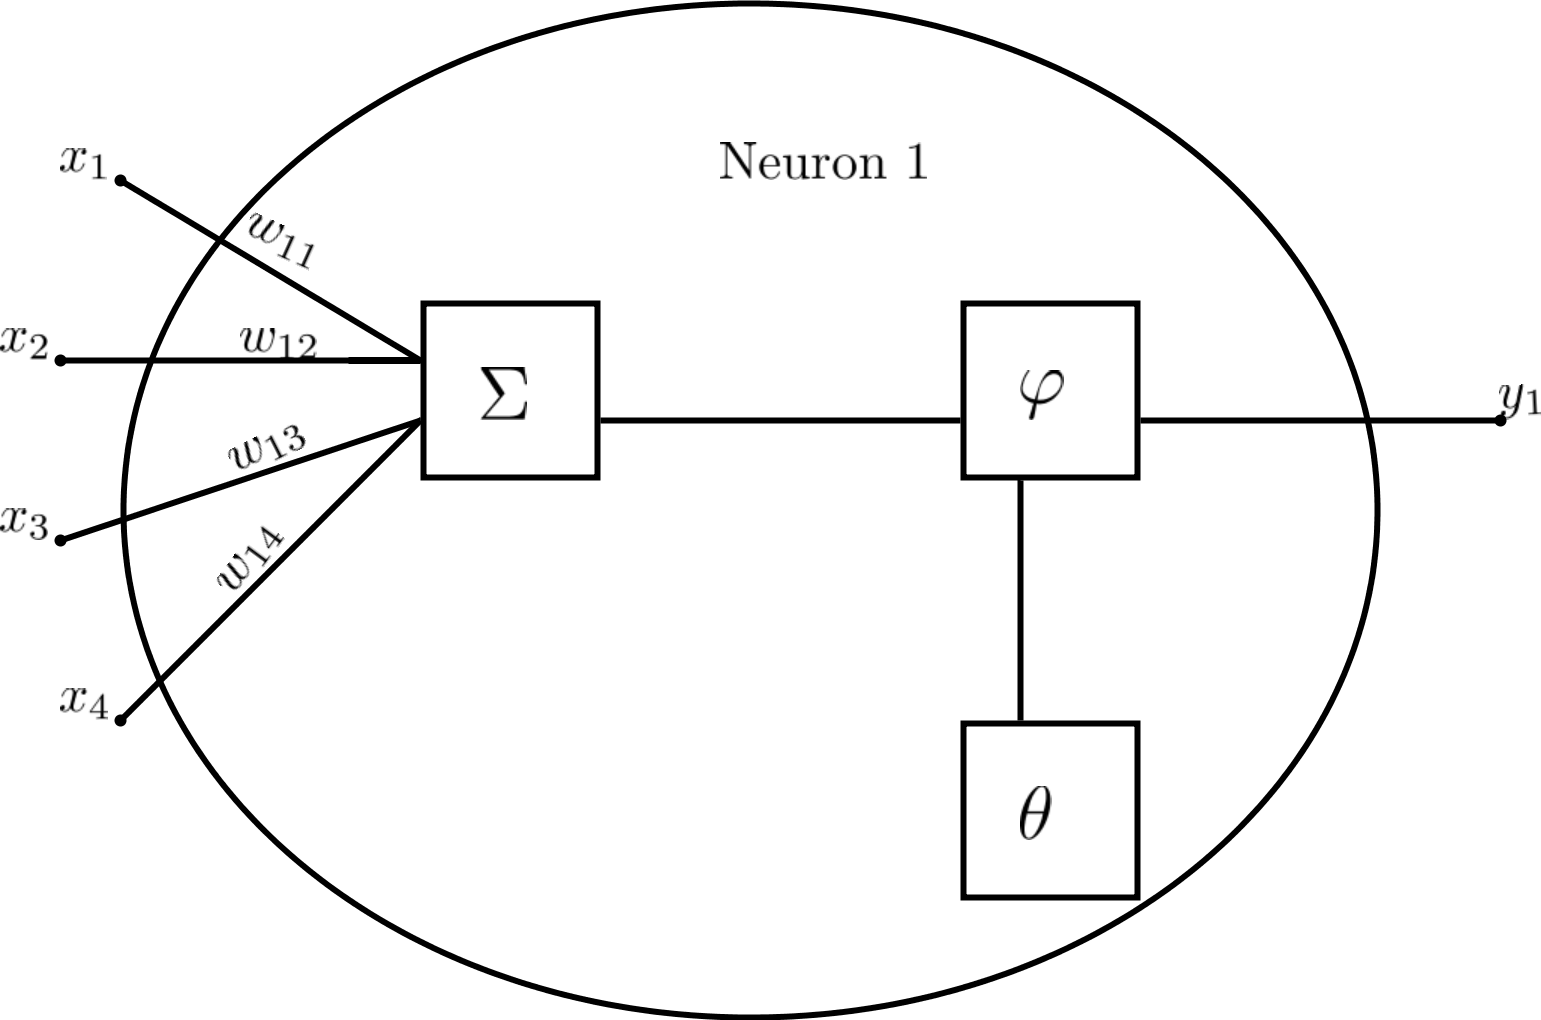
\includegraphics[width=0.7\textwidth]{images/neuron.png}
\end{figure}

\subsection{General Network Setup}
\label{sec:fund:netSetup}

A basic neural network consists of three layers: the input, a hidden layer of neurons and the output layer. Hereby, the output layer consists of as many neurons as classes that the network is trying to classify against and the one with the highest activation after entering input, is the classification output of the net.  A basic, fully-connected (referring to the connections between neurons, so fully-connected means each neuron is connected to each possible other neuron) net can be seen in Fig.~\ref{fig:net}.

\begin{figure}
\label{fig:net}
\caption{A schematic drawing of a neural network}
\centering
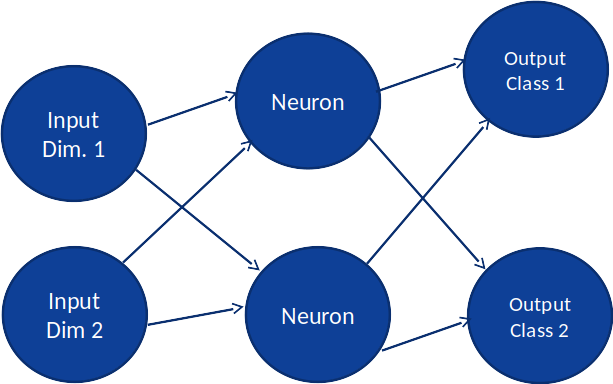
\includegraphics{images/net.png}
\end{figure}

\subsection{Network Types}
\label{sec:fund:types}

\subsubsection{Feed-Forward Neural Networks}
A basic (non-deep) \textit{Feed-Forward Neural Network} consists of three layers: the input, a hidden layer of neurons and the output layer. Feed-Forward refers to the fact, in opposition to \textit{Recurrent Neural Networks}, that connections between the neural units are not cyclic. 

In such a basic network, the output layer consists of as many neurons as classes that the network is trying to classify against and the neuron with the highest activation after entering input, is the classification output of the net.

\subsubsection{Deep Feed-Forward Neural Networks}
\textit{Deep Feed-Forward Neural Networks}, DNNs, the net-type most used in this thesis, refer to Networks that have more than one hidden layer between input and output, but still feature non-cyclic connections between neurons. DNNs have a better performance than single-hidden-layer-networks in general, but require different techniques for training. 

A common description of this phenomen is, that each hidden layer increases the level of abstraction the network can manage. E.g, in image processing, if the first layer recognizes a color in a certain pixel, then the next layer can infer more abstract characteristics from the output of the first layer. For example, after knowing a certain pixel is dark the next layer can derive that area might be the eye in a picture of a face, etc. This obviously makes more complicated classification tasks possible but also makes learning algorithms more difficult.

\subsubsection{Deep Recurrent Neural Networks}
\textit{Deep Recurrent Neural Networks}, RNNs, refer to neural networks that are DNN's but cyclic connections are allowed. This means the network can have temporal behavior, so its performance changes dynamically over time, when the state of later neurons changes and affects the neurons in previous layers.


\subsection{Learning}
\label{sec:fund:Learn}
The interesting part about Neural Networks is their ability to learn from data and improve their own performance. Improving performance in this case means that by adjusting the available parameters of the neurons part of the network, we minimize a cost function that describes the difference between an optimal output and the actual output. 

A Network can be seen to be an approximation of a function \(f^*\). So, a network trying to classify an input \(x\) into a class \(y\) approximates:
\begin{equation}
\label{eq:learn}
y=f^*(x)
\end{equation}
Then one run of the Network with parameter set \(\Theta\) gives the mapping \(y = f(x;\Theta)\) and we are trying to minimize our cost function of \(C= f^* - f\) by adjusting the set of parameters in \(\Theta\) each run.

\paragraph{Three basic approaches exist for training a network:} \hspace{0pt} \\
\begin{itemize}
\item \textit{Supervised Training}, where the optimal output for input train data is known. This means, the train data has been pre-classified by a ``teacher''. This is the method we use in this thesis and further explained below.
\item \textit{Reinforcement Training}, where the optimal input for train data is not known prior to training, but the environment gives the net feedback about its own output and good output is ``reinforced'' while bad output is discouraged.
\item \textit{Unsupervised Training}, where nothing is known about the environment and the net (often) just tries to learn the probabilistic distribution of the data.
\end{itemize}

\subsubsection{Sampling}
\label{sec:fund:Sampling}

Data for training is generally split into three sets: the training set with a size of about \(80\%\) of the total available data which is then used for the training, the development set with a size of about \(10\%\) used for evaluation of the net and adjusting different parameters without ``distorting'' the last test set which also has a size of around \(10\%\) and is used for final ``clean'' validation of the net performance.

Sampling is most commonly, as in this thesis, done using the 

\subsubsection{Supervised Training}
\label{sec:fund:ST}
Supervised Training refers to training where the optimal output for the training data is known, so a classification of the train data exists prior to training. This makes calculation of the Cost function as defined in the previous section relatively easy, as we define \(C\) as the actual difference in output of the current net with current parameter set \(\Theta\) compared to the teacher-defined classification/labeling. 

\paragraph{Mean Squared Error Function}

One way to calculate the difference between the net and the teacher-classification is by using the mean squared error, as is used in the training of nets in this thesis. If  \(t\) is the expected output and \(f(x;\Theta)\) is the actual predicted output and \(M\) the number of output neurons/classes, we define the Mean Squared Error (MSE) as:
\begin{equation}
E = 1 / 2 \sum_{j=1}^{M}(f(x;\Theta) - t)^2
\end{equation}

\paragraph{Stochastic Gradient Descent} The goal of course is to minimize the MSE as defined above by adjusting parameters for each neuron and layer (including weights to output neurons) to change the predicted output of the net.  This is done by adjusting the weights in direction of the falling gradient for each weight.
\begin{equation}
w_{i+1} = w_i - \eta \nabla E(f(x;w), t) = w_i - \eta \nabla 1/2\sum_{j=1}^M(f(x;w) - t)^2
\end {equation}

This method is called the ``Gradient Descent'', with \(\eta\) being the ``Learning Rate'', the freely adjustable speed at which the network changes and therefore learns. As calculation of this gradient for every sample in the training data set is expensive, a stochastic approach is used where only a small number of samples is used each iteration to calculate the gradient, as the relation between the change of the mean error and the value of samples is not linear. Therefore the calculation of the ´´Stochastic Gradient Descent'' (SGD) is enough to estimate the real required parameter-changes.

\paragraph{Backpropagation} While the SGD is used to calculate each iterative weight according to the falling gradient, the Backpropagation algorithm is used to calculate each weight from the total output of the net and its input. If we have neural network output vector (all output neurons together) \(t_i\), input vector (all input dimensions together) \(x_i\) and current weights \(w_i\) we can calculate \(w_{i+1}\) by calculating the SGD on the function \(w \rightarrow E(w, x_i), y_i)\).

With preceding definitions we can summarize the training algorithm of a DNN as follows:
\definecolor{green}{rgb}{0.0, 0.4, 0.13}
\lstset{captionpos=b,tabsize=3,frame=lines,keywordstyle=\color{blue},commentstyle=\color{green},stringstyle=\color{red},numbers=left,numberstyle=\tiny,numbersep=5pt,breaklines=true,showstringspaces=false,basicstyle=\footnotesize,emph={label}}
\begin{lstlisting}[label=lst:pseudo:train,caption=Pseudo Code to show the Backpropagation/SGD algorithm in Action,mathescape]
 $\displaystyle w_0 := rand()$
  do
     forEach train-sample s
        $\displaystyle f(x;w_i)$ = neural-net-output$\displaystyle(w_i, s) $ // Actual calculation using each neurons output -> Forward pass
        t = pre-classification(s)
        Error = $\displaystyle E(f(x;w_i), t)$
         $ \displaystyle w_{i+1}:=  w_i - \eta \nabla E(f(x;w), t) = w_i - \eta \nabla 1/2\sum_{j=1}^M(f(x;w) - t)^2$  //For all Weights and layers -> Backwards pass
        $\displaystyle w :=w_{i+1}$
   if ($\Delta E$ <= Threshold) break
return Net
\end{lstlisting}
